\begin{figure}[p]
  \centering
  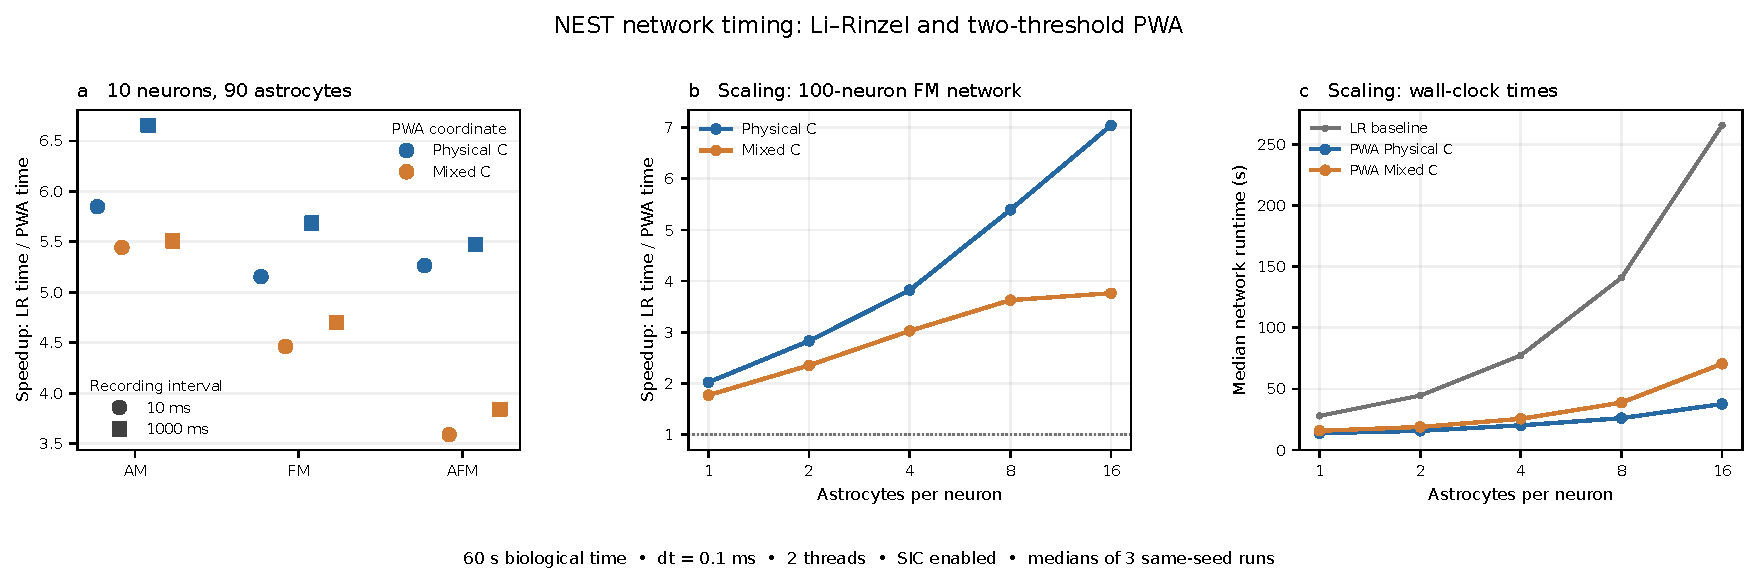
\includegraphics[width=\linewidth]{figures/figure7_nest_speed.pdf}
  \caption{Locally measured NEST closed-loop network runtimes using Li--Rinzel and two-threshold PWA astrocytes. \textbf{(a)} Speedup $t_{\rm LR}/t_{\rm PWA}$ in a 10-neuron all-to-all network with 90 astrocytes for AM, FM and AFM; marker shape indicates the astrocyte recording interval. \textbf{(b,c)} Speedup and absolute runtime in an independent 100-neuron FM network as the number of astrocytes per neuron varies. The same LR timing samples are used for both coordinate comparisons in (b,c). In both experiments $dt=0.1$ ms, biological duration is 60 s, two threads are used and SIC is enabled; no SIC was observed in the recorded AM runs. Times are medians of three \texttt{nest.Run} wall-time measurements with the same seed; speedups are ratios of these medians. The mixed FM model is an earlier archived candidate, as in Figs.~\ref{fig:period-comparison}--\ref{fig:bifurcation-comparison}. The PWA candidates are separately fitted; neuronal dynamics, SIC, recording and coordinate recovery all contribute to runtime, so the difference does not isolate the cost of a coordinate transformation.}
  \label{fig:nest-speed}
\end{figure}
